\chapter{Einleitung}
\label{ch:einleitung}

DNA Sequenzierung ist aus der biologischen und medizinischen Forschung nicht mehr wegzudenken.
Die Entwicklung immer günstigerer und leistungsstärkerer Sequenzierungsverfahren hat in den letzten Jahrzenten für einen rapiden Anstieg der zu verarbeitenden Datenmengen gesorgt.
Hinzu kommt, dass die verwendeten Verfahren nicht fehlerfrei sind, was die Verarbeitung der Daten weiter erschwert.

In dieser Arbeit wird ein Paper behandelt, in dem der Fehlerkorrekturalgorithmus FMOE vorgestellt wird.
Zu erst wird aber der Hintergrund in den Bereichen Biologie und Bioinformatik erläutert.

\section{DNA-Sequenzierung}
\label{s:dna-seq} 

%Bild: DNA-Strang -> Kopien -> Fragmente -> Reads -> Assembly -> Sequenz *?Das von Wikipedia?*
\begin{figure}[h]
\begin{center}
		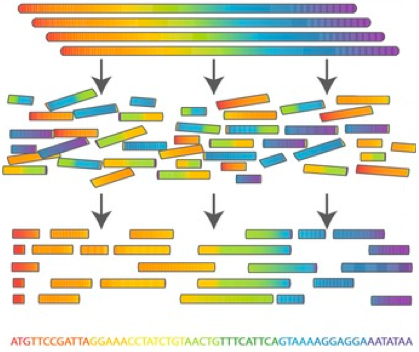
\includegraphics[width=0.45\columnwidth]{./img/shotgun_sequencing.png}
\end{center}
\caption{}
\label{fig:histogram}
\end{figure}

Das Ziel der de-novo DNA-Sequenzierung ist die Bestimmung der Nukleotidfolge in DNA ohne ein bereits bekanntes Referenzgenom.
Wo bei alten Verfahren noch alle Basen nacheinander bestimmt wurden, werden seit dem sogenannten Shotgun Sequencing viele Teilstücke der DNA parallel analysiert.
Das macht es möglich, lange DNA Stränge mit Verfahren zu sequenzieren, die nur kurze Fragmente verarbeiten können.
Gleichzeitig ermöglicht es die parallele Sequenzierung von mehreren Fragmenten, was den Vorgang extrem beschleunigt.

Die Reihenfolge der DNA-Fragmente aufrecht zu erhalten, ist möglich, aber relativ langsam und aufwendig.
Die sogenannten next-gen Sequenzierungsverfahren, welche den aktuell höchsten Durchsatz erzielen, verzichten daher darauf.
Um trotzdem auf die ursprüngliche Reihenfolge und damit auf die gesamte DNA-Sequenz zurückschließen zu können, wird das Verfahren für mehrere Kopien desselben DNA-Strangs durchgeführt.

Man trennt also mehrere Kopien des Strangs an zufälligen Positionen in ungefähr gleich lange Fragmente.
Alle Fragmente können unabhängig von einander - und damit parallel - sequenziert werden.
Das Ergebnis der Sequenzierung eines Fragments wird Read genannt.
Aufgrund der zufälligen Trennungspositionen überlappen sich die Reads häufig.
Vorausgesetzt die Abdeckung reicht aus, kann man mit den Überlappungen die Reads in die ursprüngliche Reihenfolge bringen und so die gesuchte DNA-Sequenz bestimmen.
%Fußnote Abdeckung/Coverage
Dieser Prozess heißt \textbf{Assembly}.
Wie bereits erwähnt, sind die aktuellen Verfahren zur Bestimmung der Reads nicht fehlerfrei.
Es kann zum Überspringen (Deletion) oder Vertauschen (Substitution) richtiger Basen oder zur Einfügung (Insertion) falscher Basen kommen
Kollektiv werden diese Fehler Indels genannt
%Bild: Assemblygraph *?mit und ohne Indels?*
Indels können für unterschiedlich große Probleme während der Assembly sorgen
Fehlerhafte Reads können aufgrund mangelnder Überlappung nicht korrekt eingeordnet werden, dann spricht man von fragmentierter Assembly
%satz hier drüber: wording
Größere Probleme entstehen aber, wenn Reads trotz Fehlern zu einer validen Assembly führen
Bei dieser sog. Misassembly erhält man zum Schluss unter Umständen eine valide, aber falsche Sequenz
%*?auf erhöhte komplexität der assembly bei fehlerhaften reads eingehen?*
Diese Komplikationen zu verhindern, ist Aufgabe der Fehlerkorrektur



Man sollte direkt jedes Kapitel, Unterkapitel und jede Formel mit einem Label versehen \verb+\label{}+ um eine konsistente Referenzierung im gesamten Dokument zu ermöglichen. Eine Referenzierung im Fließtext lässt sich mittels \verb+\ref{}+ umsetzen.


\section{Zeilenumbrüche und Absätze}
\label{s:zeilenumbruch} 
Zeilenumbrüche sollten im Quelltext immer mittels einer Leerzeile umgesetzt werden, um eine automatische Texteinrückung in der darauffolgenden Zeile zu ermöglichen. Dies macht das Lesen der Arbeit einfacher. Auf die Verwendung des LaTeX-Kommandos \verb+\\+ sollte verzichtet werden.


\section{Einfügen von Grafiken}
\label{s:grafik} 
Grafiken sollten mittels der \verb+\figure+-Umgebung eingebettet werden. Um die Druckqualität und Wiederverwendbarkeit der Grafiken für Vorträge, Poster, etc.\ zu erhöhen sind Vektorgrafiken (z.B.\ .eps oder .pdf) zu bevorzugen. Zur Erzeugung und Konvertierung von Vektorgrafiken ist die OpenSource Software \emph{Inkscape} zu empfehlen.

Um mehrere Bilder horizontal anzuordnen, sollte die \verb+\subfigure+-Umgebung verwendet werden. Diese Bilder können dann mit \verb+\subref+ oder \verb+\ref+ referenziert werden und erscheinen im Text als \subref{fig:subfig1} oder \ref{fig:subfig1}.

\begin{figure}
\begin{center}
	\subfigure[Das Logo]{
		
\includegraphics[width=0.45\columnwidth]{./img/wwu-logo-neu.pdf}
		\label{fig:subfig1}
	}
	\subfigure[Noch einmal das Logo]{
		
\includegraphics[width=0.45\columnwidth]{./img/wwu-logo-neu.pdf}
		\label{fig:subfig2}
	}
\end{center}
\caption{Das Logo der WWU}
\label{fig:histogram}
\end{figure}


\section{Wissenschaftliches Zitieren}
\label{s:zitat}
Für das Referenzieren von wissenschaftlicher Literatur wie Fachbüchern, Konferenzpapern und Veröffentlichungen in Wissenschaftsmagazinen gibt es unterschiedliche Konventionen. Je nach Fachrichtung weichen Layout und Zitationsstil sehr stark voneinander ab \cite{jele2010}. Wir empfehlen aus Gründen der Einheitlichkeit die Verwendung der \emph{Bibtex}-Umgebung. Die zitierte Literatur kann ausgelagert in einer Datei (z.B.: Quellen.bib) gepflegt werden und mittels des \verb+\cite+-Kommandos referenziert werden.


\section{Zusammenfassung}
\label{s:zusammenfassung}
Zum Ende eines längeren Kapitels bietet es sich häufig an eine Zusammenfassung der wichtigsten Punkte zu liefern. Dies erleichtert das Lesen und den Übergang zum nächsten Kapitel.
